\documentclass[standalone]{beamer}

\begin{document}
\section{BIT}

\begin{frame}{BIT}
  \begin{itemize}
    \item Binary Indexed Tree
    \item Fenwick Tree
    \item 樹狀數組
    \item 支援操作:單點加值、前綴求和
  \end{itemize}
\end{frame}

\begin{frame}{BIT}
  \begin{itemize}
    \item 我們有一個陣列 $a[1\ldots n]$,以及另一個陣列 $s[1\ldots n]$
    \item $s[i]$ 紀錄的是 $\sum_{j=i-lowbit(i)+1}^{i}{a[j]}$
    \item $lowbit(x)$ 的值是 $x$ 寫成二進位時最小的一個 1-bit 的值
    \item 比如說,$44 = 101100_2, lowbit(44) = 2^2 = 4$
    \item $lowbit(x) = x \& (-x)$
    \item 好抽象,來看圖吧!
  \end{itemize}
\end{frame}

\begin{frame}{BIT}
  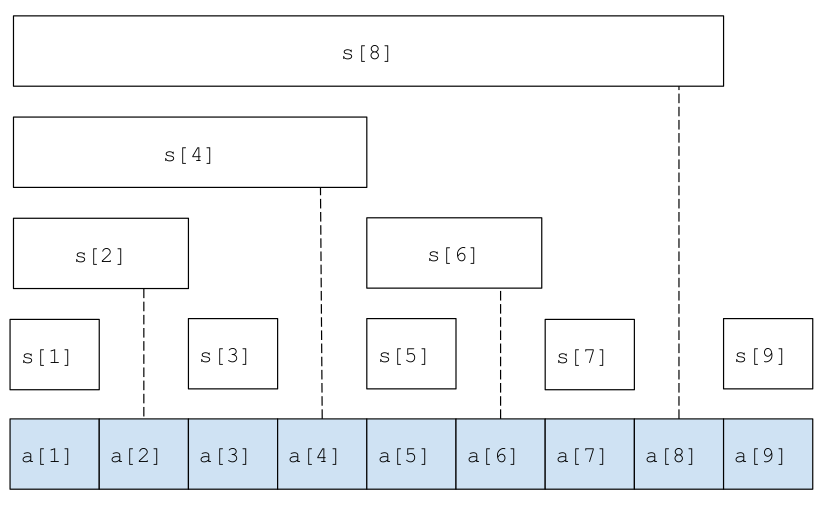
\includegraphics[width=10cm]{figures/bit.png}

  有沒有很像沒有右邊子樹的線段樹!
\end{frame}

\begin{frame}{\btitle{前綴求和}}
  \begin{itemize}
    \item 假設要求 $a[1...46]$
    \item $= s[46] + a[1...44]$
    \item $= s[46] + s[44] + a[1...40]$
    \item 有發現什麼嗎?
    \item 令 $sum(x)=a[1]+a[2]+\cdots+a[x-1]+a[x]$
    \item 前面好像就只是 $sum(x) = s[x] + sum(x - lowbit(x))$
    \item 遞迴求 $sum(x)$!
  \end{itemize}
\end{frame}

\begin{frame}[fragile]{\btitle{前綴求和}}
  \begin{minted}[breaklines]{cpp}
    int sum(int id) {
      int res = 0;
      for (int i = id; i > 0; i -= i & -i)
        res += s[i];
      return res;
    }
  \end{minted}
\end{frame}

\begin{frame}{\btitle{單點加值}}
  \begin{itemize}
    \item 假設要把 $a[46]$ 加上 $x$,把有蓋到 $46$ 的值加上去就好了
    \item 首先觀察發現有蓋到 46 的節點編號一定不小於 46 ,畢竟節點 $i$ 蓋到的區間是 $(i-lowbit(i),i]$
    \item 其實古人的智慧告訴我們,會蓋到 $i$ 的區間編號其實就是以下的序列:
    \item $\{s_0 = i, s_{k+1} = s_k + lowbit(s_k)\}$ ,一直到 $s_k > N$ 為止
      \begin{itemize}
        \item 簡單小證明:
        \item $lowbit(s_{k + 1}) > lowbit(s_k)$,所以 $s_{k + 1}$ 會覆蓋到 $s_k$ 覆蓋的範圍
        \item 而 $s_{k + 1}$ 恰好是所有覆蓋 $s_k$ 範圍中最小的那一個
      \end{itemize}
  \end{itemize}
\end{frame}

\begin{frame}[fragile]{\btitle{前綴求和}}
  \begin{minted}[breaklines]{cpp}
    void upd(int id, int x) {
      for (int i = id; i <= n; i += i & -i)
        s[i] += x;
    }
  \end{minted}
\end{frame}

\begin{frame}{\btitle{單點加值、區間求和}}
  \begin{itemize}
    \item 有了這些,就可以解決一個很常見的問題了:單點加值、區間求和
    \item 單點加值 $a_i += x$ 直接 \texttt{upd(i, x);} 就好
    \item 區間求和 $[l, r]$ 其實可以用前綴和的方式得到:\texttt{sum(r) - sum(l - 1);}
  \end{itemize}
\end{frame}

\begin{frame}{\btitle{第 K 小}}
  \begin{itemize}
    \item 假設 $a[x]$ 是存 $x$ 這個數字出現過幾次
    \item 那 $sum(i)$ 就是 $\le i$ 的元素有幾個
    \item $i$ 是集合裡第 $k$ 小的元素若且唯若 $sum(i - 1) < k$ 且 $sum(i) \ge k$
    \item 二分搜!
    \item 直接呼叫 query 二分搜是 $O(\log^2 N)$,複雜度似乎不太好
    \item 用 BIT 的結構在上面二分搜!
  \end{itemize}
\end{frame}

\begin{frame}{\btitle{第 K 小}}
  來看圖!

  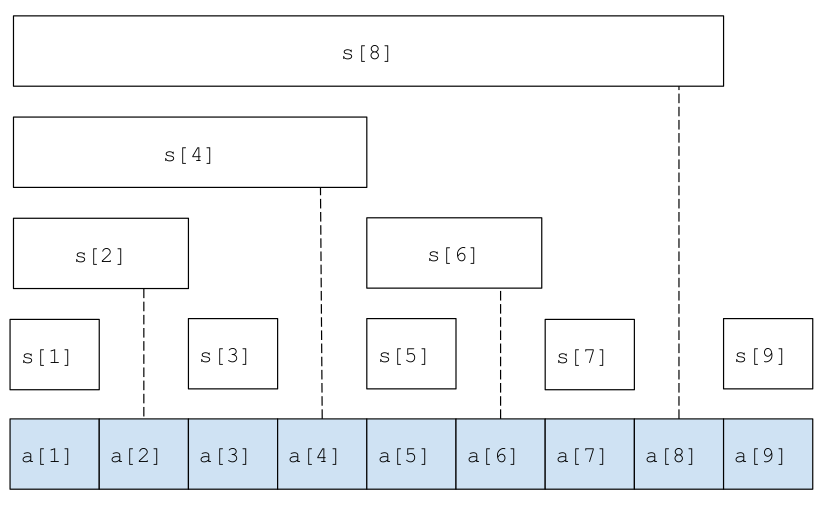
\includegraphics[width=10cm]{figures/bit.png}
\end{frame}


\begin{frame}[fragile]{\btitle{第 K 小}}
  \begin{minted}[breaklines]{cpp}
    int kth(int k) {
      int res = 0;
      for (int i = 1 << __lg(n); i > 0; i >>= 1)
        // 決定 res 應該在 [res, res + i - 1] 還是 [res + i, res + 2i - 1]
        if (res + i <= n && dat[res + i] < k) // 左邊的個數不夠,往右邊走
          k -= dat[res += i];
        // 否則就代表左邊其實是夠的,就往左邊走
      return res + 1;
    }
  \end{minted}
\end{frame}

\begin{frame}{\btitle{BIT 與差分}}
  \begin{itemize}
    \item 差分序列:$d_i = a_i - a_{i - 1}$
    \item 如果 BIT 維護差分序列的話,就可以變成支援區間加值、單點求值的資料結構
    \item $a_i = d_1 + d_2 + \ldots + d_i$
    \item 把 $a_l, \ldots, a_r$ 全部加上 $x$,相對應在差分數列上的變化其實只是 $d_l$ 加上 $x$,$d_{r+1}$ 扣掉 $x$
  \end{itemize}
\end{frame}

\begin{frame}{\btitle{總結}}
  \begin{itemize}
    \item 支援單點修改、前綴求和、查詢第 k 小的資料結構
    \item 常數很小、寫起來比線段樹簡單許多
    \item 實用!
  \end{itemize}
\end{frame}

\end{document}
